\documentclass[tikz]{standalone}
\usepackage{pgfmath}
%\usetikzlibrary{calc}

\begin{document}
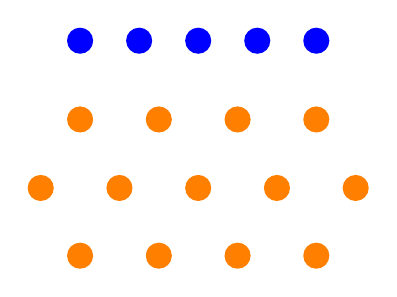
\begin{tikzpicture}

\foreach \i in {0,1,2,3,4} {
	%\shade[ball color=orange,yshift=1cm]	(\i,0) circle (0.15);
	\node[yshift=1cm,circle,fill=blue] at (\i * 0.75,0) {};
}

\foreach \i in {0,1,2,3} {
	%\shade[ball color=orange,yshift=1cm]	(\i,0) circle (0.15);
	\node[yshift=0cm,xshift=0,circle,fill=orange] at (\i,0) {};
}

\foreach \i in {0,1,2,3,4} {
	\node[yshift=-0.87cm,xshift=-0.5cm,circle,fill=orange] at (\i,0) {};
}

\foreach \i in {0,1,2,3} {
	\node[yshift=-1.73cm,xshift=0,circle,fill=orange] at (\i,0) {};
}

\end{tikzpicture}

\end{document}

